\begin{abstract}
There are many languages on the earth, and it become difficult to recognize them when it present some similarity with other language. One way to address that arise from the fields of Natural Language Processing which aim to enable computer to process human language. By developing a trigram language model on five languages, we are able to create a language identification system with an accuracy of $91.30\%$, from which we can also see which language is similar to it by the usage of the perplexity. In Addition, the Byte-Pair encoding algorithm allow us to perform an automatic subword segmentation without any knowledge of the language. This later is then used to see how similar are two language by looking on the intersection between their vocabulary which can tell us a lot of story.

\end{abstract}
\section{Introduction}
Natural Language Processing system is currently present on many devices in our daily life, from a cell phone to TV, cars. It is also used to translate a language A to a Language B, but how if we do not know what language is used A?. This problem can be solved by building a Language model based on known languages and process the A on them. To build such system, we look on how we prepare the corpus to build the model. Then the basis of the character level trigram language model and subword tokenisation system. Finally we present the results of our experimentation.

\medskip
The theory content are inspired from \cite{kamper2022nlp817, jurafsky2022speech}.
\section{Data Preprocessing: text normalization}
To build the language identification we are given five non-normalized corpus with the following language: Afrikaans (af), English (en), Deutch (nl), Xhosa (xh) and Zulu (zl).
Each of them with a normalized validation data to check and tune some hyperparameter of our model. Lastly, we have a validation set to measure the final performance of our language identification.

Thus to normalize the training data to match the form validation set we apply the following operation:
\begin{enumerate}
    \item Each paragraph is splited by detecting where we have `.', `!' or  `?' followed by space and Capital letter. Then, each sentence is placed on a single line in the normalized file data,
    \item Remove leading and trailing spaces,
    \item Replace all diacritics into its normal form, and digits by 0,
    \item Expand all abbreviation and acronyms by inserting a space,
    \item The text is then transformed into a lower case.
\end{enumerate}
To perform these operations we use the \texttt{re} package of python for regular expression and \texttt{unicodedata} for diacritics.

Once the data is ready, we can use them to build our language model.
\section{Language Modelling}
This section describes the how we build the character trigram language model, how we evaluate and generate text from it. The model will use the following vocabulary:
\begin{equation}
    \mathcal{V} = \{ \mathtt{<, >, spaces, 0, a, b, \ldots, z} \}
\end{equation}
which are obtained from the normalized corpus, where $<$ indicate the beginning of  a sentence and $>$ its end.
\subsection{Trigram model}
With a Markov assumption, given a sequence of two characters $(w_{t-2}, w_{t-1})$, a trigram model predicts the probability of a third word $w_t$ given the previous two by:
\begin{equation}
    P(w_t|w_{t-2:t-1}) = \frac{P(w_{t-2:t})}{P(w_{t-2:t-1})}
\end{equation}
and the likelihood of a given sentence  is defined by:
\begin{equation}
    P(w_{1:T})=\prod_{i=1}^{T}P(w_i|w_{i-2}w_{i-1})
\end{equation}
However, we do not have access to this true probability, as we cannot have all the possible trigrams in our training set. Therefore we have to estimate it, using maximum likelihood estimation.
\subsection{Probability estimation}
Since $P(w_t|w_{t-2:t-1})$, is not accessible we substitute it by its maximum likelihood estimation defined by:
\begin{equation}
    P_{\mathrm{MLE}}(w_t|w_{t-2:t-1}) = \frac{C(w_{t-2:t})}{C(w_{t-2:t-1})}
\end{equation}
Where $C(w_{t-2:t})$ is the count of the trigram $(w_{t-2:t})$ in the training data, and $C(w_{t-2:t-1})$ is the count of the bigram $(w_{t-2:t-1})$. Once again, some trigram will not be present, leading to a zero count, and then a zero probability for a particular sentence which does not make sense.

To handle the zero count trigram, we can use various smoothing technics, here we use the add-k smoothing which consist of adding a fractional count when computing the probability as follows:
    \begin{equation}
        P_{\mathrm{Add-k}}(w_t|w_{t-2:t-1}) = \frac{C(w_{t-2:t})+k}{C(w_{t-2:t-1})+k|\mathcal{V}|}
    \end{equation}
When $k=1$ it is called Laplace smoothing, which is the default value in our implementation. The value of $k$ is then tuned on the validation set using a grid search, and consider the one that maximize the likelihood.

Using Laplace-smoothing is fine for our language identification purpose, but it can move to punch mass to the unseen trigram, and this is one of the reasons that we tune it.

Another alternative is to use a mixture of several models, by using the probability defined by:

\begin{equation}
		P_{\mathrm{INT}}(w_t|w_{t-2:t-1}) =\lambda_iP(w_i|w_{t-2:t-1}) + \lambda_2P(w_t|w_{t-1}) + \lambda_3P(w_t)
\end{equation}
This technique is called Interpolation smoothing, the value of $\lambda_i$ can be tuned as well, and it must sum to one.

Both of these techniques are suitable for our problem, as we aim to predict in wich language is used in a given sentence.

\subsection{Model evaluation and hyperparameter tunning}
Now, with the basis of the model, we need a metric to measure how good it is. The most common metric in NLP is the perplexity, defined by the probability of the data assigned by the language model, normalized by the number of words:
\begin{equation}
    PP(W) = P(w_{1:T})^{-\frac{1}{T}} = \sqrt[T]{\frac{1}{P(w_{1:T})}}
\end{equation}
where a lower perplexity reflects a better model.
In practice we use the log probability, since the perplexity can be computed \begin{equation}
    PP(W) = P(w_{1:T})^{1/T} = 2^{-\frac{1}{N}\log_2 P(w_{1:T})}
with:\end{equation}
In our implementation we use the natural log, so the two is replaced by $e$.
Additionally, minimizing the perplexity is equivalent to maximizing the probability, and we use this fact to optimize our hyperparameter.
\subsection{Text Generation}
With the hyperparameter-tuned models, we can now generate text character by character. The code was designed to generate text from nothing or from a specific starting text. The text generation process is as follows:
\begin{itemize}
\item With a starting text: Split the text into a list of characters and add the starting marker '<' at the beginning.
\item From nothing: We start with the starting sentence, then we use the bigram model to form the first two characters, i.e., $(<, \bullet)$.

Repeat the until we meet the ending markers $>$:
\begin{itemize}
\item Compute all $p(x|w_{t-2}w_{t-1})$, for all $x\in\mathcal{V}$
\item Normalize these probabilities to ensure they form a valid probability distribution.
\item Use \texttt{np.random.multinomial} to sample the next character according to the normalized probabilities.
\end{itemize}
\end{itemize}
Note that the process described above is also used for the bigram model at the beginning if we do not specify any starting character.
The probability is computed according to the specific smoothing method.


Another utility of this metric is to look how similar a language A on language B. We can perform that by consider a corpus from A and compute the perplexity on the language model B, and vice versa. If the two languages are similar, it should yield lower perplexity on both sides, otherwise it l be high.
\section{Language identification}
this section described how we use our set of trigram models to identify the language for a given sentence by doing the following steps:
\begin{itemize}
    \item Compute the perplexity of the sentence using each of the trained language models.
    \item The predicted label (language) is then determined by the model with the lowest perplexity.
\end{itemize}
Then we apply that on the whole test set in order to determine the accuracy of our language identification. The accuracy is computed by counting the number of correct language.
\section{Byte-Pair Encoding and Language Similarity}
We have already mentioned that the perplexity can be used to analyse the similarity of two languages. Here, we compare the vocabulary generated by the Byte-Pair Encoding (BPE) algorithm to see how similar they are.

The BPE is an algorithm that allows automatic subword token learning from a given training corpus by following the process bellow:
\begin{enumerate}
    \item Initialization:
    \begin{itemize}
    \item Initialize the tokens at the character level.
    \item Create the initial vocabulary $\mathcal{V}$ using the unique characters from the tokens.
    \end{itemize}

    \item Repeat for $k$ times:
    \begin{itemize}
        \item Find the most frequent pair of adjacent tokens $t_L, t_R$ in the corpus.
        \item Create a new token $t_{new} = t_L + t_R$ (merge the pair).
        \item Add the new token $t_{new}$ to the vocabulary $\mathcal{V}$.
        \item Replace all occurrences of $t_L, t_R$ with $t_{new}$ in the corpus.
        \item Record the merge into the history.
    \end{itemize}
\end{enumerate}

The resulting vocabulary $\mathcal{V}$ will have $k + |$Initial Characters$|$ tokens after the $k$ iterations.

If the algorithm is run for a very large number of merges, the vocabulary may contain complete words from the training corpus, which may not be the most useful representation.

Therefore, the appropriate number of merges should be chosen to obtain a compact set of sub-word units that can effectively represent the original text corpus. This allows the model to handle rare and out-of-vocabulary words by decomposing them into these learned sub-word units.
\section{Result and Discussion}
In this ection we show the results obtained from our implemetation and related discussion.
\subsection{Perplexity}
The perplety is a way to measure the performace of our language models, the figure bellow show the perplexity of each model on each language.
\begin{figure}[H]
    \centering
    \begin{subfigure}[t]{0.5\linewidth}
        \centering
        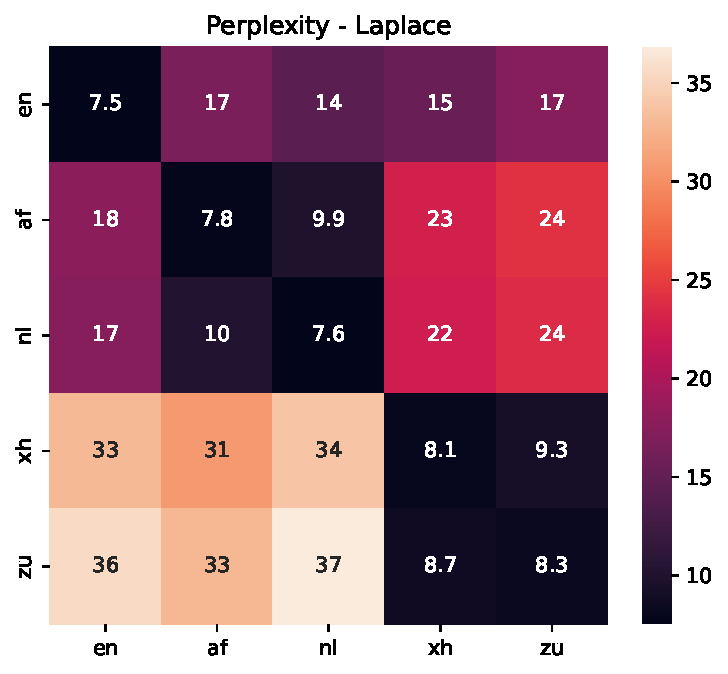
\includegraphics[width=\linewidth]{./figures/laplace.pdf}
        \caption{Laplace smoothing}
    \end{subfigure}%
    \begin{subfigure}[t]{0.5\linewidth}
        \centering
        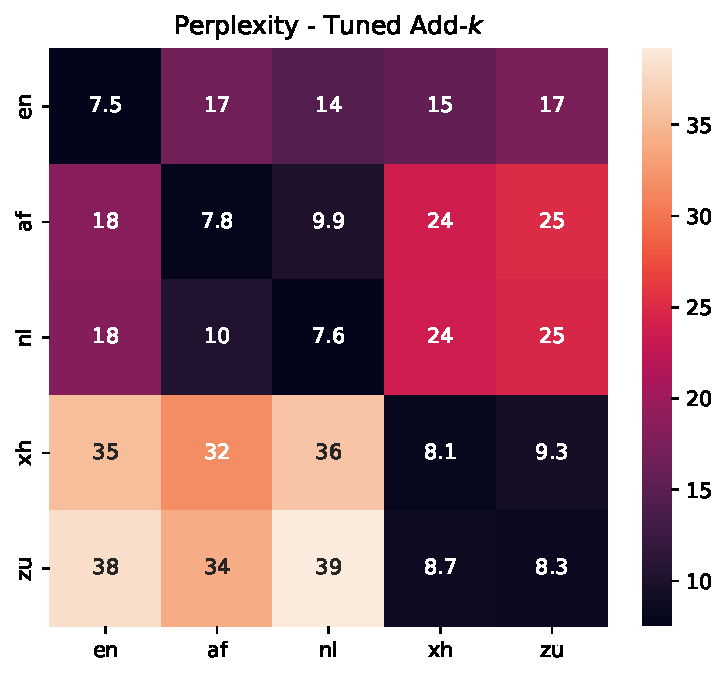
\includegraphics[width=\linewidth]{./figures/add_k.pdf}
        \caption{Add-$k$ smoothing}
    \end{subfigure}\\
    \caption{Perplexity of the models on each validation for Add-$k$}
    \label{fig:add-k}
\end{figure}
\begin{figure}[H]
	\centering
	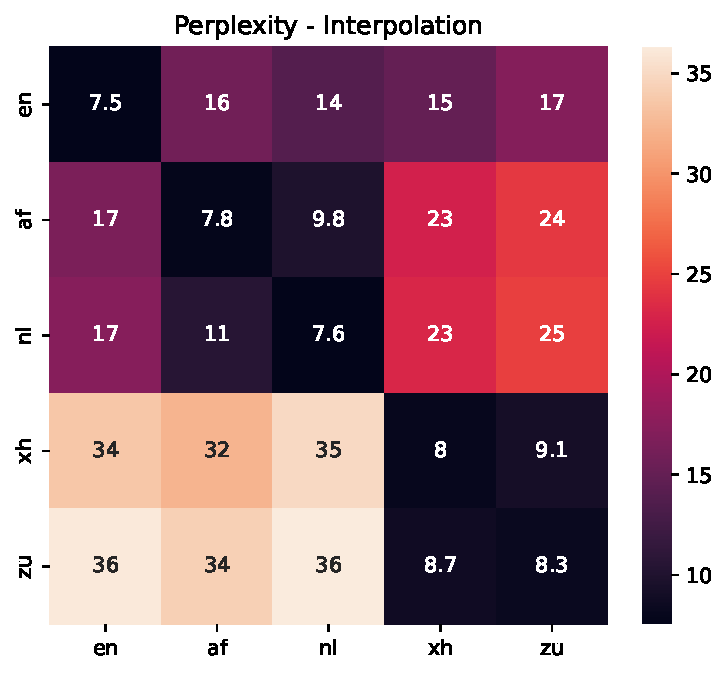
\includegraphics[width=0.5\linewidth]{./figures/inter.pdf}
	\caption{Perplexity computed with the interpolation smoothing on each validation set}
	\label{fig:interp}
\end{figure}
The values in the Figure \ref{fig:add-k} and \ref{fig:interp} are  similar (they may differ by a small number only).
The add-$k$ is the tuned version of the Laplace smoothing, where the value of $k$ are
$(\mathtt{en}: 0.505),
	(\mathtt{af}: 0.64),
	(\mathtt{nl}: 0.55),
	(\mathtt{xh}: 0.37)$ and
	$(\mathtt{zu}: 0.46)$. For the Interpolation smoothing we manually tweaked the values, and set the $\lambda_1=0.9,\ \lambda_2=0.075$, and $\lambda_3 = 0.025$ for each language.

Since we have the similar value of perplexities, than mean they will give similar results. So we will focus on the result given by the Add-k models only.


Firstly these value suggest that the each model perform well on the respective language used to build them, on the diagonal. Secondly, it also show us the similarity between Xhosa and Zulu, Afrikaans and Ducth.

\subsection{Text generation}
In this era, language model can generate well formed sentences, so we will look on an example generated by out trigram language models.

Firstly let us look on the probability of all possible trigram with an history 'th' using the English Language model. These probabilities are presented in the Table \ref{tab:add-alpha-smoothing}.
\begin{table}[h]
	\centering
	\begin{minipage}{0.48\linewidth}
	\begin{tabular}{lr}
	\toprule
	Symbol & Probability \\
	\midrule
	$P(e|t,h)$ & 0.6801 \\
	$P( |t,h)$ & 0.10159 \\
	$P(a|t,h)$ & 0.08302 \\
	$P(i|t,h)$ & 0.04469 \\
	$P(o|t,h)$ & 0.03796 \\
	$P(r|t,h)$ & 0.03386 \\
	$P(n|t,h)$ & 0.00461 \\
	$P(s|t,h)$ & 0.00333 \\
	$P(>|t,h)$ & 0.00286 \\
	$P(u|t,h)$ & 0.00239 \\
	$P(y|t,h)$ & 0.00198 \\
	$P(w|t,h)$ & 0.00071 \\
	$P(d|t,h)$ & 0.00064 \\
	$P(l|t,h)$ & 0.00057 \\
	$P(m|t,h)$ & 0.00044 \\
	\bottomrule
	\end{tabular}
	\end{minipage}\hfill\begin{minipage}{0.48\linewidth}
	\begin{tabular}{lr}
	\toprule
	Symbol & Probability \\
	\midrule
	$P(c|t,h)$ & 0.0003 \\
	$P(t|t,h)$ & 0.00024 \\
	$P(p|t,h)$ & 0.00017 \\
	$P(f|t,h)$ & 0.0001 \\
	$P(b|t,h)$ & 0.0001 \\
	$P(h|t,h)$ & 3e-05 \\
	$P(g|t,h)$ & 3e-05 \\
	$P(0|t,h)$ & 3e-05 \\
	$P(v|t,h)$ & 3e-05 \\
	$P(<|t,h)$ & 3e-05 \\
	$P(k|t,h)$ & 3e-05 \\
	$P(x|t,h)$ & 3e-05 \\
	$P(j|t,h)$ & 3e-05 \\
	$P(z|t,h)$ & 3e-05 \\
	$P(q|t,h)$ & 3e-05 \\
	\bottomrule
	\end{tabular}
	\end{minipage}

	\vspace*{0.1cm}
	\caption{Add-k English LMs, probabilities for $(\bullet|t, h)$ }
	\label{tab:add-alpha-smoothing}
\end{table}
We observe in the Table \ref{tab:add-alpha-smoothing} that the most comm trigram `the' have the highest probability in our model. That make sense because it is among the most common word in English. The followed by `th', `tha', `thi', and `tho`, we can expect that results if we have a good model, as these trigram appear often in English word.


The following sentence are generated by the English model: $\mathtt{<tests mat che mort werne>}$ started with `test' and $\mathtt{<trate chism the foolle ped goln haversaines epare>}$ started from an empty string. It seems to  not have any meaning, as we look look on a character level, which is based on the trigram so it is rare to obtain a word with a real meaning but it ca appear.
\subsection{Language Identification}
Now, let us look on the result of the language identification using the trigram model.
\begin{figure}[H]
	\centering
	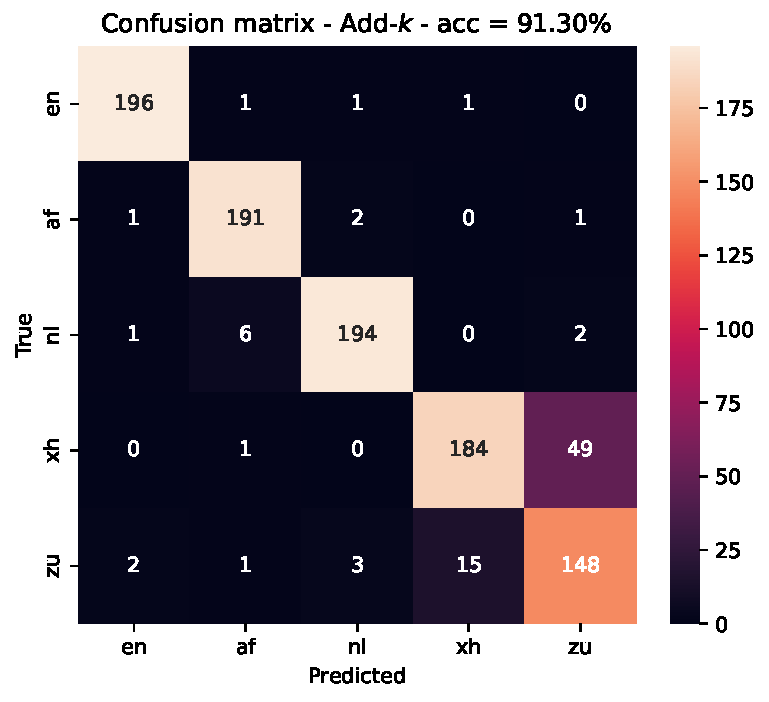
\includegraphics[width=0.75\linewidth]{./figures/acc_lang.pdf}
	\caption{Accuracy of the Language Identification}
	\label{fig:lang-acc}
\end{figure}
From the Figure \ref{fig:lang-acc}, we observe that the model perform well on identifying the language on the test set.  However it suffer to make the difference between Xhosa and Zulu, as these language are very similar (next section, for more detailed reference).

\subsection{Language Similarity}
After running the Byte-Pair Encoding algorithm for 100 merges, the first ten merges on each language are shown in the Table \ref{tab:merge-history}.
\begin{table}[H]
	\centering
	\scalebox{0.9}{\begin{tabular}{clllll}
		\toprule
		i & en & af & nl & xh & zl \\
		\midrule
		1 & e+\_ $\rightarrow$ e\_ & e+\_ $\rightarrow$ e\_ & n+\_ $\rightarrow$ n\_ & a+\_ $\rightarrow$ a\_ & a+\_ $\rightarrow$ a\_ \\
		2 & s+\_ $\rightarrow$ s\_ & n+\_ $\rightarrow$ n\_ & e+\_ $\rightarrow$ e\_ & e+\_ $\rightarrow$ e\_ & i+\_ $\rightarrow$ i\_ \\
		3 & t+h $\rightarrow$ th & e+r $\rightarrow$ er & e+n\_ $\rightarrow$ en\_ & i+\_ $\rightarrow$ i\_ & e+\_ $\rightarrow$ e\_ \\
		4 & d+\_ $\rightarrow$ d\_ & d+ie\_ $\rightarrow$ die\_ & t+\_ $\rightarrow$ t\_ & o+\_ $\rightarrow$ o\_ & n+g $\rightarrow$ ng \\
		5 & n+\_ $\rightarrow$ n\_ & s+\_ $\rightarrow$ s\_ & d+e\_ $\rightarrow$ de\_ & a+n $\rightarrow$ an & a+n $\rightarrow$ an \\
		6 & e+r $\rightarrow$ er & 0+\_ $\rightarrow$ 0\_ & s+\_ $\rightarrow$ s\_ & k+u $\rightarrow$ ku & o+\_ $\rightarrow$ o\_ \\
		7 & a+n $\rightarrow$ an & a+n $\rightarrow$ an & a+a $\rightarrow$ aa & n+g $\rightarrow$ ng & 0+\_ $\rightarrow$ 0\_ \\
		8 & t+\_ $\rightarrow$ t\_ & e+l $\rightarrow$ el & 0+\_ $\rightarrow$ 0\_ & e+l $\rightarrow$ el & k+u $\rightarrow$ ku \\
		9 & th+e\_ $\rightarrow$ the\_ & i+e\_ $\rightarrow$ ie\_ & e+l $\rightarrow$ el & i+n $\rightarrow$ in & t+h $\rightarrow$ th \\
		10 & i+n $\rightarrow$ in & d+ie\_ $\rightarrow$ die\_ & e+n $\rightarrow$ en & e+n $\rightarrow$ en & e+l $\rightarrow$ el \\
		\bottomrule
	\end{tabular}}
		\caption{Ten first merge on each language}
	\label{tab:merge-history}
\end{table}
For English (the only one that have some expertise), we see that the merge were performed on the most common bigram and word ending in this table. For example on the 9th we can already se `the\_' where `th' have been merged on the 3rd iteration.



Now let us look on the similarity on the vocabulary composed by 128 types generated by the BPE. The results are summarised in the Figure \ref{fig:similarity}. It suggests that (Zulu-Xhosa) and (Dutch-Afrikaans) share a significant amount of common vocabulary, likely due to their close linguistic relationship. On the other hand, Afrikaans and English, as well as Dutch and English, share a smaller percentage of their vocabulary, indicating a more distant relationship.

\begin{figure}[H]
	\centering
	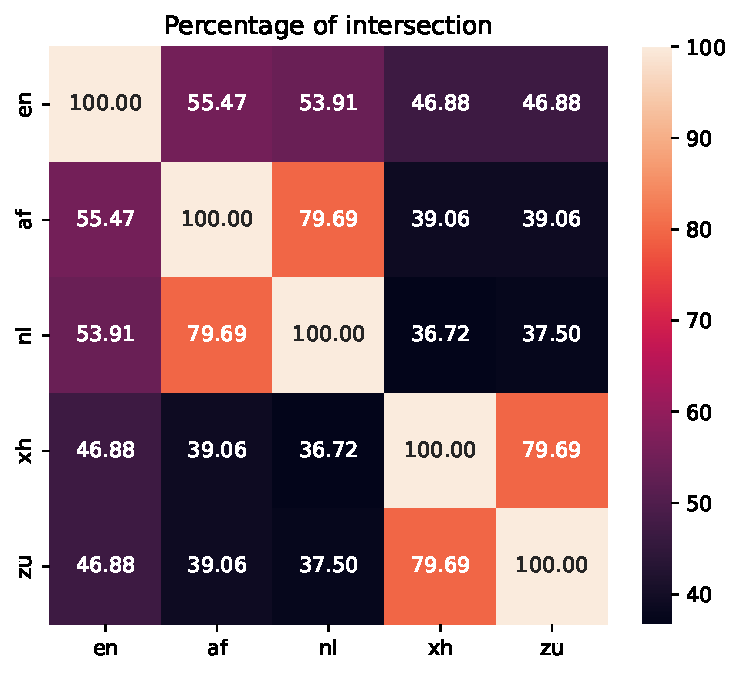
\includegraphics[width=0.75\linewidth]{./figures/intersection_cmf.pdf}
	\caption{Percentage of intersection of the vocabulary of each language}
	\label{fig:similarity}
\end{figure}

As I do not know the underlying history on these languages (except English), I did not really have an expected results. But after some discussion with friend an a look on \cite{elinguisticsnet2023compare} that quantify the genetic proximity of two languages.
Thus, these results make a lot so sense. From \cite{elinguisticsnet2023compare}, we have the following measure of Genetic proximity:
\begin{itemize}
	\item Zulu and Xhosa: 20.6 (Closely related)
	\item Dutch and Afrikaans: 2.8 (Very closely related)
	\item Afrikaans and English: 22.5 (Closely related)
	\item Dutch and English: 21.5 (Closely related)
	\item Xhosa and  Dutch: not detected (not related)
\end{itemize}

As explained there the scale are interpreted as follow:
\begin{itemize}
\item 1-30: Highly related languages. Protolanguage\footnote{Common `ancestor'} between several centuries and approx. 2000 years.
\item 30-50: Related languages. Protolanguage approx. between 2000 and 4000 years.
\item 50-70: Remotely related languages. Protolanguage approx. between 4000 and 6000 years. Chance interference increases with values above 60-62.
\item 70-78: Very remotely related languages. Protolanguage approx. older than 6000 years - but high potential of interference with chance resemblance.
\item 78-100: No recognizable relationship: the few resemblances measured are more likely to be due to chance than to common origin.
\end{itemize}

These result of genetic proximity support the result that we obtain from our vocabulary sharing percentage. Since comparing vocabulary  is effectively one way to measure the similarity of two language. The BPE, is tool that allow us to have a better segmentation of the words without any knowledge of the language. Additionally, these measure reflect the perplexity values measured on the validation set. Because, on the similar language the perplexity value are close and low, and on distant language we have high perplexity, which a reason of the accuracy measured on Xhosa and Zulu for the language identification.


\section{Conclusion}
In this work, we have seen how to prepare a corpus to build a trigram models, and use the trigram model to identify the language used in a given sentence. Our language system achieve an accuracy of $91.30\%$, the results suffer from the similarity between language especially between Xhosa and Zulu. Finally, we use the Byte-Pair Encoding algorithm to measure the similarity cross-language by looking the vocabulary overlapping, giving a results that reflect the finding in the language identification system.